% !TEX TS-program = pdflatexmk

\documentclass[modern]{aastex61}

\usepackage{acronym}
\usepackage{amsmath}
\usepackage{amssymb}

\newcommand{\chieff}{\chi_\mathrm{eff}}
\newcommand{\dd}{\mathrm{d}}
\newcommand{\diff}[2]{\frac{\dd #1}{\dd #2}}
\newcommand{\fixme}[1]{\textcolor{red}{FIXME: #1}}
\newcommand{\pali}{p_\mathrm{ali}}
\newcommand{\piso}{p_\mathrm{iso}}

\newcommand{\checkme}[1]{\textcolor{red}{#1}}

\newcommand{\OOneSigmaIsoAligned}{\checkme{1.7}}
\newcommand{\OOneOddsIsoAligned}{\checkme{0.044}}
\newcommand{\OTwoSigmaIsoAlignedMin}{\checkme{3.0}}
\newcommand{\OTwoOddsIsoAlignedMin}{\checkme{0.0012}}

\begin{document}

\acrodef{BBH}{binary black hole}
\acrodef{BH}{black hole}
\acrodef{EM}{electromagnetic}
\acrodef{GW}{gravitational wave}

\title{Distinguishing Between Spin-Aligned and Isotropic Binary Black
  Hole Populations in Advanced LIGO}

\author[0000-0003-1540-8562]{Will M. Farr}

\affiliation{Birmingham Institute for Gravitational Wave Astronomy,
  University of Birmingham, Birmingham, B15 2TT, United Kingdom}

\author[0000-0002-6100-537X]{Simon Stevenson}

\affiliation{Birmingham Institute for Gravitational Wave Astronomy,
  University of Birmingham, Birmingham, B15 2TT, United Kingdom}

\author{M. Coleman Miller}

\affiliation{Department of Astronomy and Maryland Center for Theory
  and Computation, University of Maryland, College Park MD
  20742, United States}

\author[0000-0002-6254-1617]{Alberto Vecchio}

\affiliation{Birmingham Institute for Gravitational Wave Astronomy,
  University of Birmingham, Birmingham, B15 2TT, United Kingdom}

\author[0000-0002-6134-8946]{Ilya Mandel}

\affiliation{Birmingham Institute for Gravitational Wave Astronomy,
  University of Birmingham, Birmingham, B15 2TT, United Kingdom}

\author{Friends}

\email{w.farr@bham.ac.uk,miller@astro.umd.edu,av@star.sr.bham.ac.uk,imandel@star.sr.bham.ac.uk}

\begin{abstract}
  The first direct detections of \acp{GW} from merging \acp{BBH} in
  the last year open a unique window into the formation environment of
  these systems.  One promising signature of the formation environment
  is the angular distribution of the \ac{BH} spins; systems formed
  through dynamical interacions among already-compact objects are
  expected to have isotropic spin orientations while binaries from
  pairs of stars born together are more likely to have spins aligned
  with the binary orbit as a consequence of their joint evolution
  toward a \ac{BBH} system.  By considering existing \ac{GW}
  measurements of $\chieff$, the best-measured combination of spin
  parameters, in the three likely binary black hole detections
  GW150914, LVT151012, and GW151226, we show that the data already
  exhibit a $\OOneSigmaIsoAligned\sigma$ ($\OOneOddsIsoAligned$ odds
  ratio) preference for an isotropic angular distribution amongst a
  suite of models for the spin distribution.  By considering the
  effect of an additional 10 detections (a possible outcome of the
  ongoing second observing run of Advanced LIGO) drawn from the
  various models in the suite we show that such an agumented data set
  would enable at least a $\OTwoSigmaIsoAlignedMin\sigma$
  ($\OTwoOddsIsoAlignedMin$ odds ratio) distinction between the
  isotropic and aligned models, and in most cases better than
  $5\sigma$ ($2.9 \times 10^{-7}$ odds ratio).
\end{abstract}

\acresetall{}

\section{Introduction}

This is a reference dump at the moment.  

We should be sure to discuss \citet{Rodriguez2016} here; they note the
small $\chieff$ of GW150914, but only in the context of looking for a
single system that is \emph{definitely} formed from dynamical
interactions; obviously, the population provides a more stringent
origin test.

We find much higher resolving power than \citet{Vitale2015}, probably
because they focus on measurements of spin \emph{angles}, using a
mixture model comprising an aligned and isotropic component.

In order to perform our analysis we need to select models for the 
distribution of the dimensionless spin parameters of stellar-mass black 
holes.  Data for such model selection is sparse.  \citet{2015PhR...548....1M} 
give current estimates of the spin parameters for stellar-mass black holes, 
obtained using disk reflection and/or disk continuum methods.  

Most of the systems studied are low-mass X-ray binaries (i.e., the donor star 
has a mass $M_{\rm donor}<1~M_\odot$) rather than the high-mass X-ray binaries 
that are likely to be the progenitors of double black hole binaries.  In 
addition, there are substantial systematic errors that can complicate either 
type of analysis (see \citealt{2015PhR...548....1M} for a discussion). Nonetheless, 
if we take the reported spin magnitudes as representative then we find that there 
is a preference for high spins; for example, 14 of the 19 systems with reported 
spins have spin parameters in excess of 0.5.  The masses and spin parameters of 
stellar-mass black holes are unlikely to be altered significantly by accetion 
(low-mass donors simply do not have enough mass and high-mass donors have a very 
short phase in which they transfer mass; a variant of this long-standing argument 
was presented by \citealt{1999MNRAS.305..654K}).  Thus the current spin parameters 
probably are close to their values upon core collapse.  We emphasize, however, 
that the specific processes involved in the production of black hole binaries 
could alter the spin distribution of those holes: for example, close tidal 
interactions could spin up the core, or stripping of the envelope could reduce the 
available angular momentum.

With this in mind, we do our analysis using three straw-man spin distributions for 
spin parameters from $a/M=0$ to 1: flat ($P(a/M)=1$); rising ($P(a/M)=2a/M$); and 
falling ($P(a/M)=2(1-a/M)$).  These are not meant to represent any particular 
physical model, and indeed neither observations nor population synthesis codes 
can authoritatively suggest {\it any} particular spin distribution.  This does, 
however, allow us to see how sensitive the $\chieff$ distribution is to spin alignment 
models given uncertainties about the spin magnitudes.


\section{Model Selection Formalism}
\label{sec:formalism}

This is currently pasted from the iPython notebook:

Cole had a great idea, the thrust of which is the following: assume
that you have some distribution for the spin magnitudes of black holes
(and it is common to the more- and less-massive BH in any binary).
The distribution of $\chieff$ that is implied by this magnitude
distribution differs depending on whether you assume that the angular
distribution is isotropic or aligned.  In general, isotropic angular
distributions concentrate more of the $\chieff$ distribution near
zero, since that is where most of the angular phase space is.  Here we
derive the distributions for $\chieff$ under various reasonable, yet
straw-man assumptions.

First, $\chieff$ is defined by
\begin{equation}
\chieff = \frac{c}{GM} \left( \frac{s_1^z}{m_1} + \frac{s_2^z}{m_2}
\right) = \frac{1}{M} \left( m_1 a_1^z + m_2 a_2^z \right)
\end{equation}
where the $\hat{z}$ axis is aligned with the orbital angular momentum,
$s_{1,2}$ are the spin angular momentum of the components of the
binary, and $a_{1,2}$ are the spin parameters of the black holes in
the binary.

First we derive the distribution for $a^z$ when we know the
distribution for $a$ and the angular distribution is (a) isotropic and
(b) aligned.  First isotropic: Then $a^z$ is equal to the product of
$a$ with a uniform random variable on $[-1,1]$ ($\iota = \cos \theta$,
with $\theta$ the colatitude on a sphere).  Therefore
\begin{equation}
  p\left( a^z \right) = \int_{-1}^{1} \dd \iota \, \int_0^1 \dd a \, \delta\left( a^z - a \iota \right) \frac{p(a)}{2} = \int_{-1}^{1} \dd \iota \, \int_0^1 \dd a \, \frac{\delta\left( a - \frac{a^z}{\iota} \right)}{\left| \iota \right|} \frac{p(a)}{2}.
\end{equation}
Now, noting that the distribution of $a^z$ is an even function, assume
that $a^z > 0$; since $0 \leq a \leq 1$, we must have $\iota \geq a^z$
if the $\delta$-function is to be "activated," so
\begin{equation}
p\left( a^z \right) = \int_{a^z}^1 \dd \iota \, \frac{p\left( \frac{a^z}{\iota} \right)}{2 \iota}.
\end{equation}
The even assumption implies 
\begin{equation}
p\left( a^z \right) = \int_{\left| a^z \right|}^1 \dd \iota \,
\frac{p\left( \frac{\left|a^z\right|}{\iota} \right)}{2 \iota}
\end{equation}
When the angles are aligned, we have
\begin{equation}
p\left( a^z \right) = \begin{cases}
p_a\left(a^z \right) & a^z > 0\\
0 & \mathrm{otherwise}
\end{cases}.
\end{equation}
In other words, the distribution of $a^z$ follows $a$ when $a^z$ is
positive, and is zero otherwise.

For example, when the magnitude distribution is flat, $p(a) = 1$, the
isotropic angle assumption implies that
\begin{equation}
\piso\left( a^z \right) = -\frac{\log \left| a^z \right|}{2},
\end{equation}
while the aligned assumption implies that
\begin{equation}
\pali\left( a^z \right) = \begin{cases}
1 & a^z > 0 \\
0 & a^z < 0
\end{cases}
\end{equation}

If the mass ratio, $q$, (recall: $0 \leq q \leq 1$) is zero, this is
all we need; if not, then
\begin{equation}
\chieff = \frac{1}{1+q}\left(a_1^z + q a_2^z\right),
\end{equation}
and the distribution is given by a convolution of the distributions
for $a^z$:
\begin{equation}
p\left(\chieff \right) = \int_{-1}^1 \dd a_1^z \, \int_{-1}^1 \dd a_2^z \, \delta\left( \chieff - \frac{1}{(1+q)} \left[a_1^z + q a_2^z \right]\right) p\left( a_1^z\right) p\left(a_2^z\right),
\end{equation}
which becomes, after some manipulation,
\begin{equation}
p\left(\chieff \right) = \int_{-1}^1 \dd a_1^z \, \int_{-1}^1 \dd a_2^z \, \delta\left( a_1^z + q a_2^z - (1+q)\chieff \right) (1+q) p\left( a_1^z\right) p\left(a_2^z\right),
\end{equation}
and more manipulation:
\begin{equation}
p\left(\chieff \right) = \int_{\max\left(-1, \frac{(1+q)\chieff - 1}{q} \right)}^{\min\left(1, \frac{(1+q)\chieff+1}{q}\right)} \dd a_2^z \, (1+q) p\left(a_2^z\right) p\left((1+q)\chieff - q a_2^z \right).
\end{equation}

Here we will consider three models for the spin magnitude distribution
of the two \ac{BH} spins.  The ``flat'' model assumes that magnitudes
are drawn uniformly in $[0, 1]$:
\begin{equation}
  \label{eq:flat-def}
  p(a) = 1.
\end{equation}
This model is maximally uncertain about the spin magnitude.  The
increasing distribution is meant to be more consistent with the
existing \ac{EM} observations of \acp{BH} in X-ray binaries
\citep{Miller2015}
\begin{equation}
  \label{eq:increasing-def}
  p(a) = 2a.
\end{equation}
The ``decreasing'' distribution is meant to be more consistent with
the observed low-spins in the existing \ac{GW} detections
\citep{O1-BBH}, with
\begin{equation}
  \label{eq:decreasing-def}
  p(a) = 2(1-a).
\end{equation}

This is not going to be analytic, even if we specialise to $q = 1$
(equal mass); though a good check of the math is that it works out to
the above single-spin distribution when $q=0$.  We should just
simulate the distribution empirically.  The result appears in Figure
\ref{fig:chieff-distribution-models}

\begin{figure}
  \plotone{../plots/chi-eff-distributions}
  \caption{\label{fig:chieff-distribution-models} The models for the
    distribution of $\chieff$ considered in this paper.  In all models
    we assume that the binary mass ratio $q \equiv m_1/m_2 = 1$.  The
    ``flat'' model (blue curves) for the spin magnitudes is defined in
    Eq.\ \eqref{eq:flat-def}; the ``increasing'' model (green curves)
    for the spin magnitudes is defined in Eq.\
    \eqref{eq:increasing-def}; and the ``decreasing'' model (red
    curves) is defined in Eq.\ \eqref{eq:decreasing-def}.  Solid lines
    give the $\chieff$ distribution under the assumption that the
    orientations of the spins are isotropic; dashed lines give the
    distribution under the assumption that both objects' spins are
    aligned with the orbital angular momentum.}
\end{figure}

LIGO measures $\chieff$ better than any other spin parameter, but
still with significant uncertainty, so we need to properly incorporate
measurement uncertainty in our analysis; thus our analysis must be
\emph{hierarchical}.  In a hierarchical analysis, we assume that each
event has a true, but unknown, value of the effective spin, drawn from
the population distribution, which may have some parameters $\lambda$;
then the system is observed, represented by the likelihood function,
which results in a distribution for the true effective spin (and all
other paremeters describing the system) consistent with the data.
Combining, the *joint* posterior on each system's $\chieff^i$
parameters and the population parameters $\lambda$ implied by a set of
observations each with data $d^i$, is
\begin{equation}
  p\left( \left\{ \chieff^i \right\}, \lambda \mid \left\{ d^i \right\} \right) \propto \left[ \prod_{i=1}^{N_\mathrm{obs}} p\left(d^i \mid \chieff^i \right) p\left( \chieff^i \mid \lambda \right) \right] p\left(\lambda\right).
\end{equation}

The components of this formula are
\begin{itemize}
\item The GW (marginal) likelihood, $p\left(d \mid \chieff\right)$.
  "Marginal" because we are (implicitly) *integrating* over all
  parameters of the signal but $\chieff$.  Note that it is the
  *likelihood*, not the *posterior* that matters for the hierarchical
  analysis; if we are given posterior distributions or posterior
  samples, we need to re-weight to "remove" the prior and obtain the
  likelihood.
\item The population distribution for $\chieff$,
  $p\left( \chieff \mid \lambda \right)$.  This function can be
  parameterised by population-level parameters, $\lambda$.  (In the
  cases discussed above, there are no parameters for the population.)
\item The prior on the population-level parameters, $p(\lambda)$.
\end{itemize}
If we don't care about the individual event $\chieff$ paremetrs, we
can integrate them out, obtaining
\begin{equation}
  p\left( \lambda \mid \left\{ d^i \right\} \right) \propto \left[ \prod_{i=1}^{N_\mathrm{obs}} \int \dd \chieff^i \, p\left(d^i \mid \chieff^i \right) p\left( \chieff^i \mid \lambda \right) \right] p\left(\lambda\right).
\end{equation}
If we are given posterior samples of $\chieff^{ij}$ ($i$ labels the
event, $j$ labels the particular posterior sample) drawn from an
analysis using a prior $p\left( \chieff \right)$, then we can
approximate the integral by an re-weighted average of the population
distribution over the samples (here $p\left( \chieff^{ij} \right)$ is
the prior used to produce the posterior samples):
\begin{equation}
  p\left( \lambda \mid \left\{ d^i \right\} \right) \propto \left[ \prod_{i=1}^{N_\mathrm{obs}} \frac{1}{N_i} \sum_{j=1}^{N_i} \frac{p\left( \chieff^{ij} \mid \lambda \right)}{p\left( \chieff^{ij} \right)} \right] p\left(\lambda\right).
\end{equation}

In a fully-spinning `LALInference` analysis, our prior for $\chieff$
is given by the combination of a flat prior in the spin magnitudes
with an isotropic prior in angles.

\section{Results From O1}
\label{sec:O1}

We approximate the posteriors on $\chieff$ for the three \ac{GW}
events reported in \cite{O1-BBH} by Gaussians with the same median and
90\% range reported in that paper.  Our approximations are shown in
Figure \ref{fig:O1-posteriors}.

\begin{figure}
  \plotone{../plots/chi-eff-mock-posteriors}
  \caption{\label{fig:O1-posteriors} ``Mock'' posteriors from the O1
    observations.  We approximate the posteriors reported in
    \citet{O1-BBH} with Gaussians with the same median and 90\%
    range.}
\end{figure}

The hierarchical analysis described in Section \ref{sec:formalism}
results in the odds ratios shown in Figure \ref{fig:O1-odds}.  The
best-fitting isotropic model (``decreasing'') is favoured over the
best-fitting aligned model (``decreasing'') by an odds ratio of
$\OOneOddsIsoAligned$, which corresponds to $\OOneSigmaIsoAligned$.

%\begin{figure}
%  \plotone{../plots/O1-model-selection}
%  \caption{Odds ratios among our six models using the approximations
%    to the posteriors on $\chieff$ from the O1 observations shown in
%    Figure \ref{fig:O1-posteriors}.  The flat, increasing, and
%    decreasing spin magnitude distributions (``F'', ``I'', ``D'';
%    Eqs.\ \eqref{eq:flat-def}, \eqref{eq:increasing-def},
%    \eqref{eq:decreasing-def}) are paired with isotropic and aligned
%    angular distributions (``I'', ``A'').  The most-favoured isotropic
%    model has a decreasing distribution of spin magnitudes, as does
%    the most-favoured aligned model.  The odds ratio between these
%    models is $\OOneOddsIsoAligned$, or $\OOneSigmaIsoAligned\sigma$.}
%  \label{fig:O1-odds}
%\end{figure}

\begin{figure}
  \plotone{../plots/Wills_evidence_ratio_figure_with_mixture_models.png}
  \caption{Odds ratios among our models using the approximations
    to the posteriors on $\chieff$ from the O1 observations shown in
    Figure \ref{fig:O1-posteriors}.  The flat, increasing, and
    decreasing spin magnitude distributions (``$\mathrm{F}$'', ``$\mathrm{I}$'', ``$\mathrm{D}$'';
    Eqs.\ \eqref{eq:flat-def}, \eqref{eq:increasing-def},
    \eqref{eq:decreasing-def}) are paired with isotropic, aligned
    angular distributions (``$\mathrm{I}$'', ``$\mathrm{A}$''), as well as a mixture model of the two (``$\mathrm{M}$'').  The most-favoured models have a decreasing distribution of spin magnitudes.  The odds ratio between these
    models is $\OOneOddsIsoAligned$, or $\OOneSigmaIsoAligned\sigma$.}
  \label{fig:O1-odds}
\end{figure}

\section{Mixture model}

BBHs can form as the end point of isolated binary evolution \cite{refs}, or dynamically in dense stellar environments \cite{refs}. The spin misalignments of BBHs is a signature of their formation mechanism; binaries formed through isolated binary evolution are expected to have their spins aligned with the orbital angular momentum, whilst those formed dynamically are expected to have an isotropic distribution.

Rate uncertainties for both of these formation scenarios are large enough that we do not know a priori which will dominate the LIGO detection rate. In the previous section we have shown that a model with isotropic spin directions and 'decreasing' spin magnitudes is favoured by the data.

In this section we assume that the true distribution of BBH spin-orbit misalignments observed by LIGO is a mixture of binaries formed through isolated binary evolution (with aligned spins) and dynamical formation (with isotropic spins). 

%
\begin{figure}
\centering
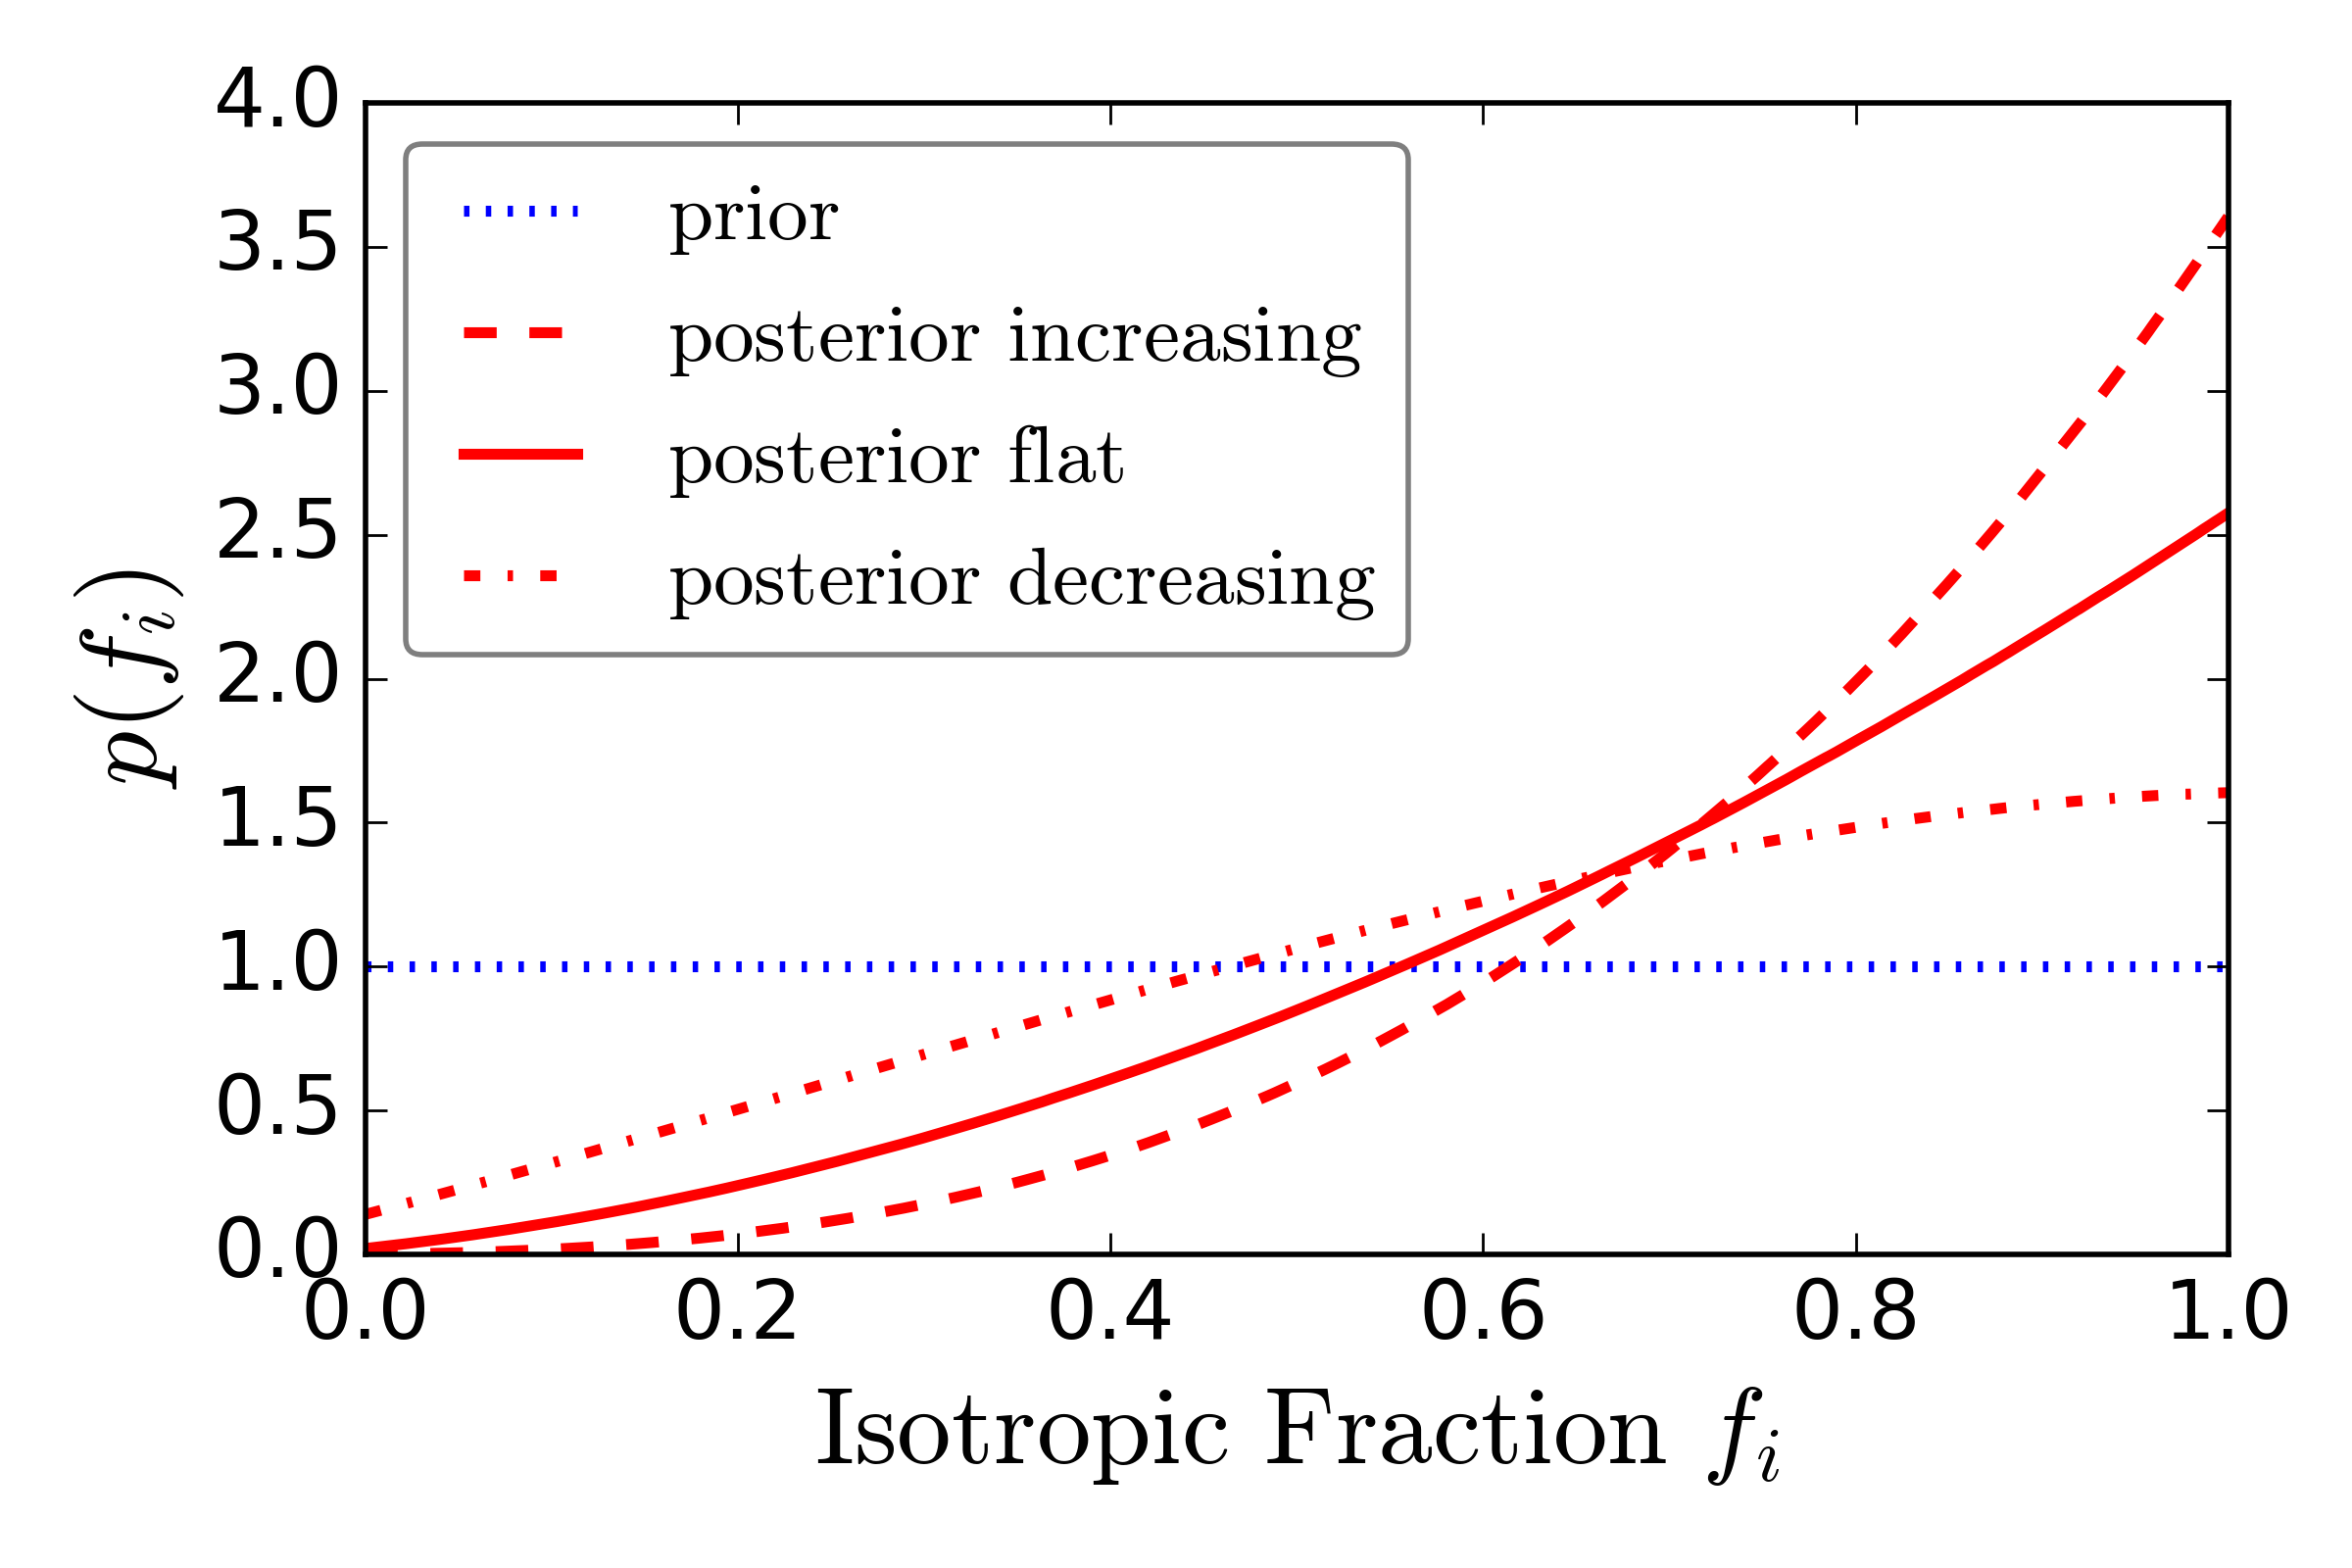
\includegraphics[width=0.45\textwidth]{../plots/posterior_on_isotropic_fraction.png}
\caption{\textbf{Fraction of the BBH population coming from an isotropic distribution} The dotted (blue) line shows the flat prior on the fraction of BBHs coming from an isotropic distribution $f_i$. The solid (red) line shows the posterior after O1, assuming that all BHs have their spin magnitude drawn from a uniform distribution. The dashed line assumes a `increasing' distribution $p(a) = 2a$ for BH spin magnitudes, whilst the dot-dash line assumes a `decreasing' distribution $p(a) = 2(1-a)$. We see that regardless of our assumption regarding BH spin magnitudes, there is a preference for a large fraction coming from an isotropic distribution.}
\label{fig:mixture_fraction_posterior}
\end{figure}
%

%-- could also use the cumulative posterior
%%
%\begin{figure}
%\centering
%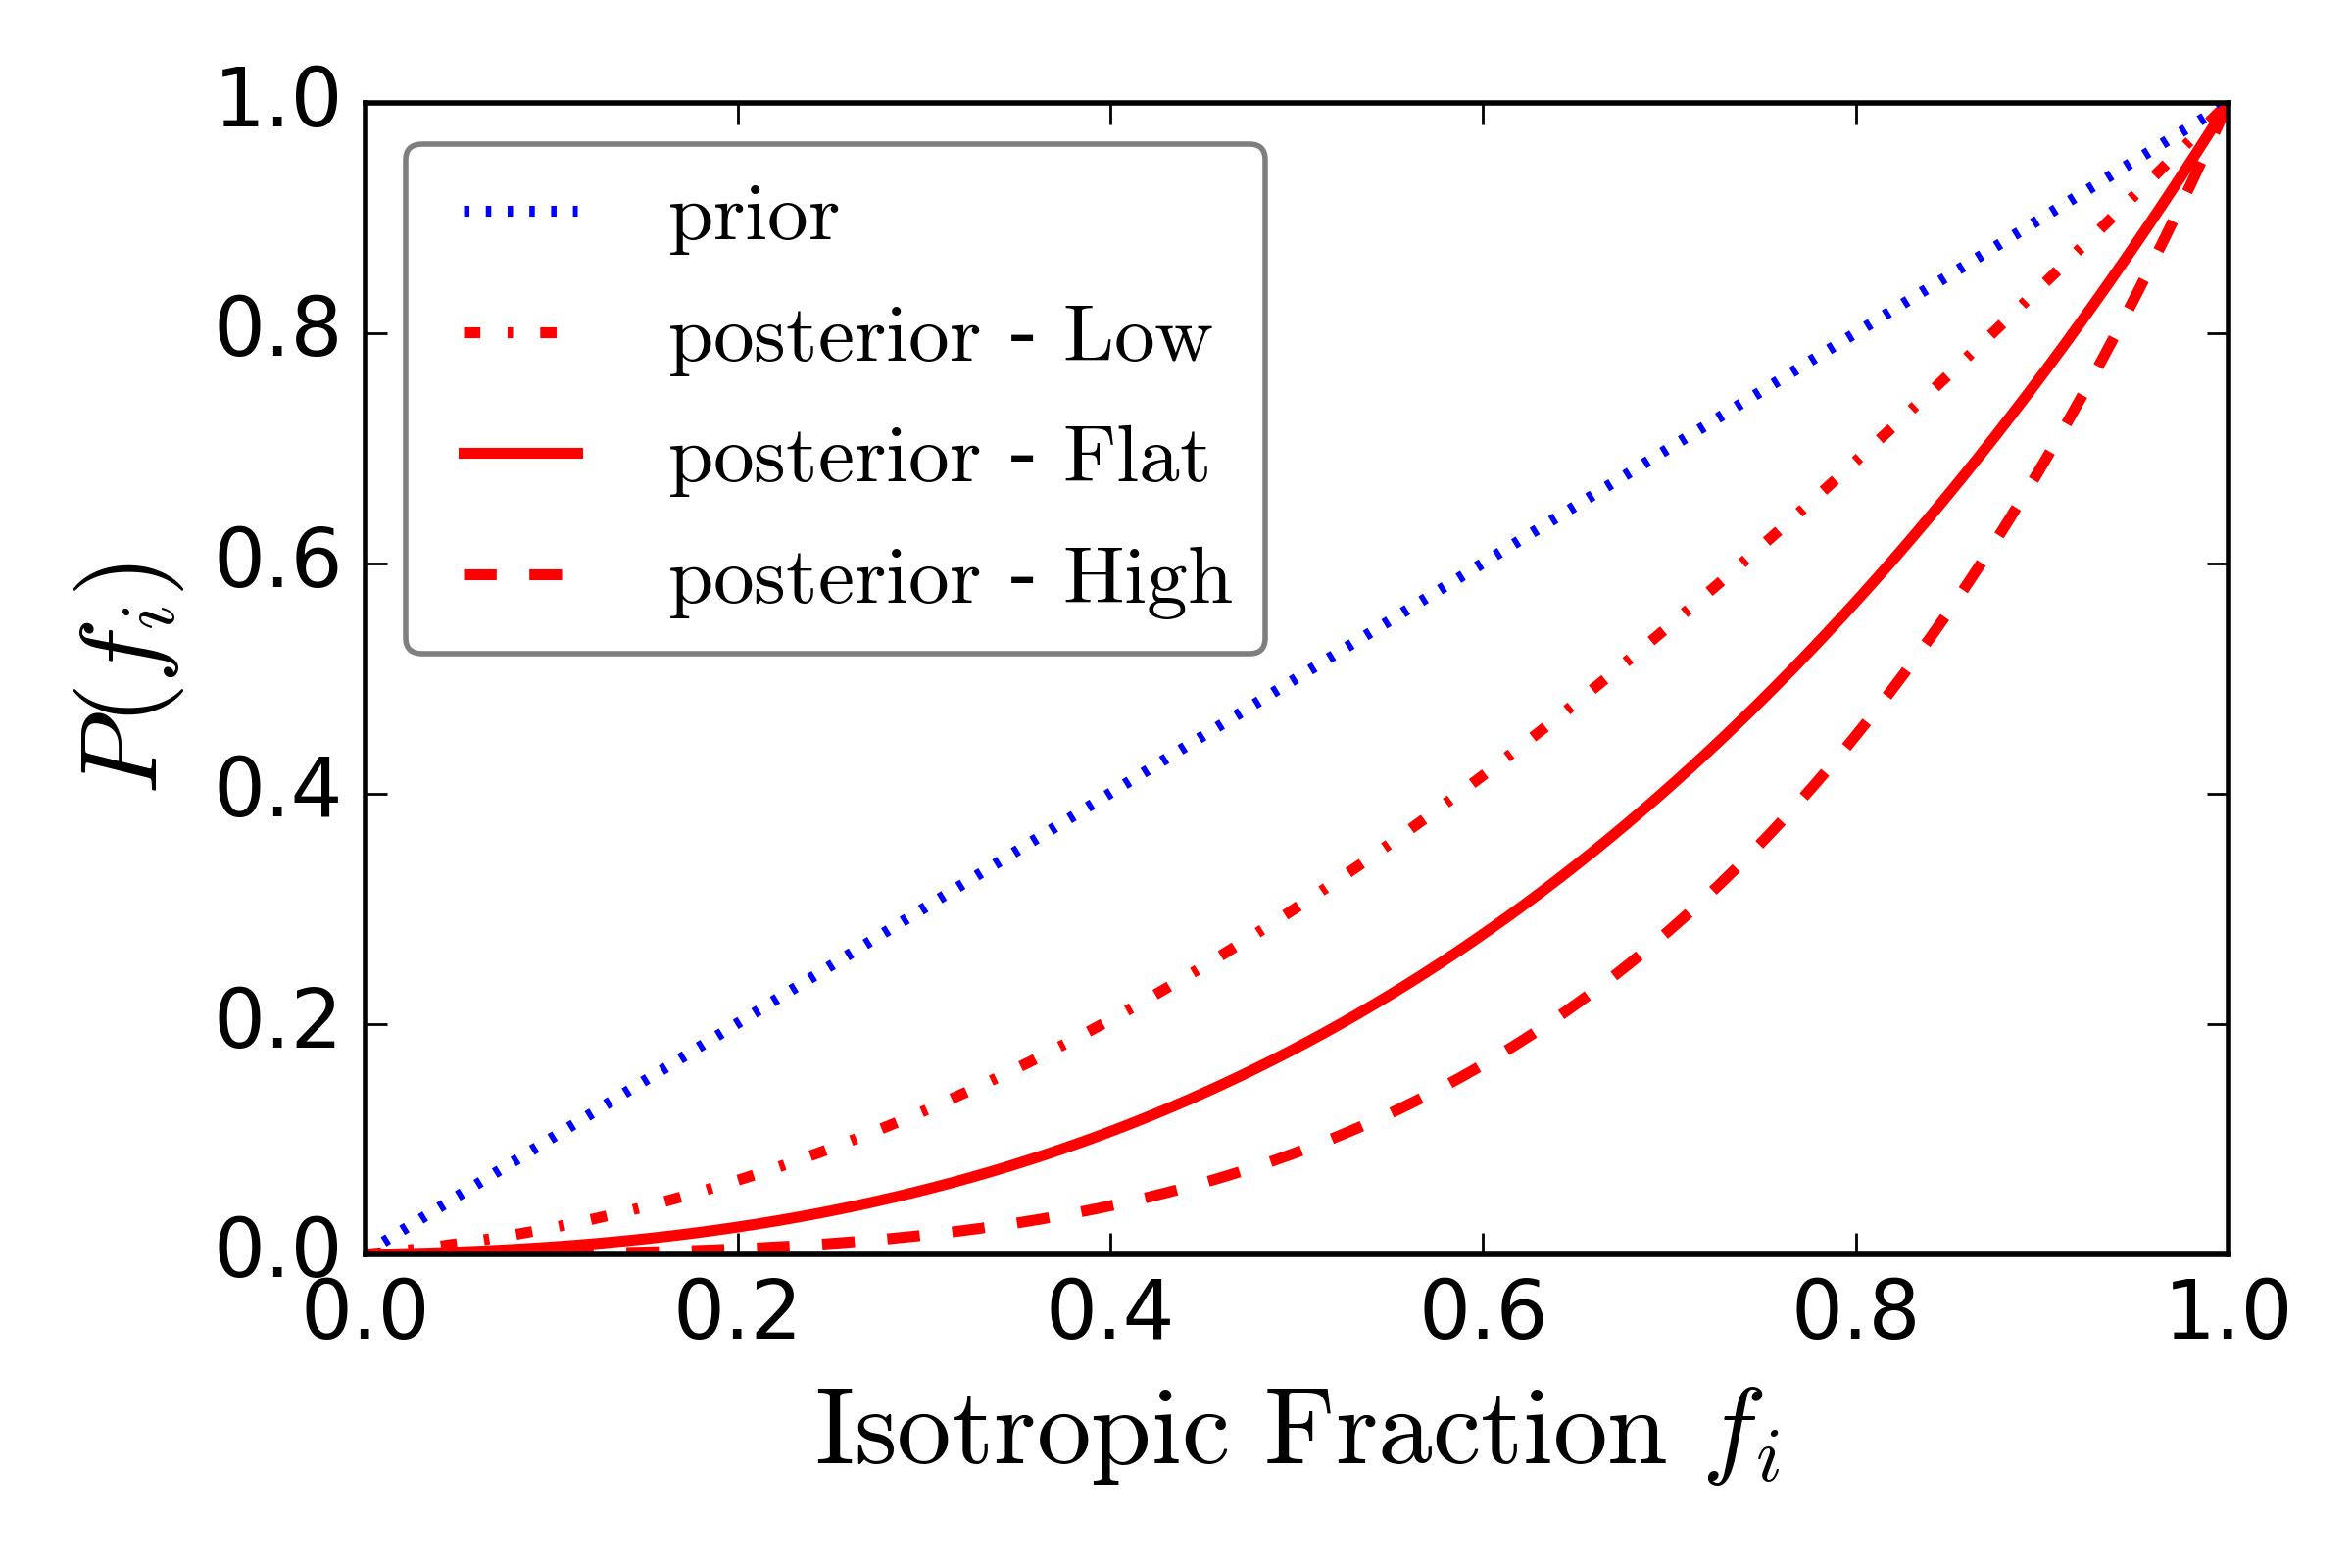
\includegraphics[width=0.45\textwidth]{../plots/isotropic_fraction_cumulative_posterior.png}
%\caption{\textbf{Fraction of the BBH population coming from an isotropic distribution} The dotted (blue) line shows the cumulative distribution for the flat prior on the fraction of BBHs coming from an isotropic distribution $f_i$. The solid (red) line shows the cumulative distribution for the posterior after O1, assuming that all BHs have their spin magnitude drawn from a uniform distribution. The dashed line assumes a `increasing' distribution $p(a) = 2a$ for BH spin magnitudes, whilst the dot-dash line assumes a `decreasing' distribution $p(a) = 2(1-a)$. We see that regardless of our assumption regarding BH spin magnitudes, there is a preference for a large fraction coming from an isotropic distribution.}
%\label{fig:mixture_fraction_posterior}
%\end{figure}
%

We fit a mixture model (labelled model 'M') where a fraction $f_i$ ($f_i=\lambda$ in the derivations above) of BBHs have spins drawn from an isotropic distribution, whilst a fraction $1 - f_i$ have their spins aligned with the orbital angular momentum. We assume a flat prior on the fraction $f_i$. To test the robustness of our result, we vary the distribution we assume for BH spin magnitude distributions as with the aligned and isotropic models. We use the `uniform', `increasing' and `decreasing' distributions introduced in Section X, assuming all BHs have their spin magnitude drawn from the same distribution. We calculate the posterior given by EquationX plot the posterior distribution/cumulative posterior in Figure~\ref{fig:mixture_fraction_posterior}. We find the mean fraction of BBHs coming from an isotropic distribution is 0.63, 0.71 and 0.78 assuming the `decreasing', `uniform' and `increasing' distributions for spin magnitudes respectively, compared to the prior mean of 0.5. The lower 90\% limits are 0.26, 0.39 and 0.52 respectively, compared to the prior of 0.1. Thus, irrespective of our ignorance of the BH spin magnitude distribution, we find that the current O1 LIGO observations constrain the majority of BBHs to have their spins drawn from an isotropic distribution. 

If we assume that the subpopulation of BBHs with isotropically distributed spin orientations corresponds to a subpopulation of dynamically formed BBHs, our result suggests that the majority of merging BBHs observed by LIGO are formed dynamically, rather than through isolated binary evolution.

The evidence ratios of these models to the isotropic distribution with uniform spin magnitudes are 0.85, 0.39 and 0.19. Thus we cannot rule out a mixture with the current data. 


\section{Predictions for the Future}

See Figure \ref{fig:O2-predictions}.

\begin{figure}
  \plotone{../plots/six-way-O2-model-selection}
  \caption{\label{fig:O2-predictions} Distribution of odds ratios
    predicted with 10 additional observations above the three
    discussed in Section \ref{sec:O1}.  Each panel corresponds to
    additional observations drawn from one of the $\chieff$
    distribution models.  The model from which the additional
    observations are drawn is outlined in red.  The height of the blue
    bar gives the median odds ratio relative to the model from which
    the additional observations are drawn; the green line gives the
    68\% ($1 \sigma$) symmetric interval of odds ratios over 1000
    separate draws from the model distribution.  The closest ratio
    between the most-favoured isotropic model and the most-favoured
    aligned model is $\OTwoOddsIsoAlignedMin$, corresponding to
    $\OTwoSigmaIsoAlignedMin\sigma$ preference for the correct angular
    distribution; most models result in more than $5\sigma$ preference
    for the correct angular distribution.  Because the three
    observations from Section \ref{sec:O1} are included in each data
    set the ``correct'' model is not necessarily preferred over the
    others, particularly when that model uses the ``increasing''
    magnitude distribution, which is strongly dis-favoured from the O1
    observations alone.}
\end{figure}

\section{Conclusion}

\bibliography{AlignedIsotropicGW}

\end{document}

